\message{ !name(sample.tex)}\documentclass{beamer} % "Beamer" is a word used in Germany to mean video projector. 

\usetheme{Montpellier} % Search online for beamer themes to find your favorite or use the Berkeley theme as in this file.

\usecolortheme{rose}
\usepackage[utf8x]{inputenc}
\usepackage[english,russian]{babel}
\usepackage{color} % It may be necessary to set PCTeX or whatever program you are using to output a .pdf instead of a .dvi file in order to see color on your screen.
\usepackage{graphicx} % This package is needed if you wish to include external image files.
\usepackage{amsmath}
\usepackage{ulem}
\theoremstyle{definition} % See Lesson Three of the LaTeX Manual for more on this kind of "proclamation."
\newtheorem*{dfn}{A Reasonable Definition}               

\newcommand{\twopartdef}[4]
{
	\left\{
		\begin{array}{ll}
			#1 & \mbox{если } #2 \\
			#3 & \mbox{если } #4
		\end{array}
	\right.
}
\title{Оптимизация параметров стратегий поиска объектов на море}
\author{Антон Ковшаров} 
\institute{Санкт-Петербургский национальный исследовательский университет \\ информационных технологий, механики и оптики}
%\date{mm 15, 2015} 

\AtBeginSection[]  % The commands within the following {} will be executed at the start of each section.
{
\begin{frame} % Within each "frame" there will be one or more "slides."  
\frametitle{Содержание} % This is the title of the outline.
\tableofcontents[currentsection]  % This will display the table of contents and highlight the current section.
\end{frame}
} %  Do not include the preceding set of commands if you prefer not to have a recurring outline displayed during your presentation.

\begin{document}
\message{ !name(sample.tex) !offset(-2) }


\beamertemplatetransparentcoveredmedium
\begin{frame} 
\titlepage
\end{frame}

\section{Постановка задачи}
\begin{frame}
  \frametitle{Цель работы}
   Построить маршрут поиска объекта максимизирующий вероятность его обнаружения. Фиксированы: \\
\begin{itemize}
  \item распределениe вероятности (зависимость от времени)
  \item параметры средства поиска
  \item стратегия поиска - ``параллельное галсирование''
\end{itemize}
\end{frame}

\begin{frame}
  \frametitle{Распределение вероятности}
\begin{columns}
\column{.6\textwidth}
\includegraphics<+>[width=\textwidth]{pics/pic03-1.png}
\includegraphics<+>[width=\textwidth]{pics/pic03-2.png}
\includegraphics<+>[width=\textwidth]{pics/pic03-3.png}
\includegraphics<+->[width=\textwidth]{pics/pic03-4.png}
\column{.4\textwidth}
\setbeamercovered{dynamic}
\begin{itemize}
\item<.(-3)>{Начальное распределение}
  \begin{itemize}
     \item Нормальное распределение
     \item Равномерное распределиние
  \end{itemize}
\item<.(-2)-.(0)>{Эволюция распределения (диффузия)}
\end{itemize}
\end{columns}
\end{frame}

\begin{frame}[t]
\only<1>{Распределение вероятности}
\only<2->{\sout{Распределение вероятности}\\}
\only<2->
{
Распределение частиц\\
\pause
\begin{itemize}
  \pause
\item частица - гипотеза положения объекта поиска
  \pause
\item перемещение частиц с течением времени
  \pause
\item сбор частиц средством поиска
  \pause
\item больше собранных частиц --- больше вероятность обнаружить объект
\end{itemize}
}
\end{frame}

\begin{frame}
  \frametitle{Параметры распределения}
\begin{itemize}
\item $A_{t_0} : R^2 \to R $ --- начальное распределения (аппроксимируется матрицей)
\item $f(A_t, \Delta t) = A_{t+\Delta t}$ --- функция изменения распределения
\end{itemize}
\end{frame}

\begin{frame}
  \frametitle{Параметры средства поиска}
\begin{itemize}
\item $p_0$ --- начальное положение средства поиска
\item $v$ --- cкорость средства поиска
\item $r$ --- радиус обнаружения средства поиска (все частицы попавшие в круг радиуса обнаружения считаются ``собранными'')
\end{itemize}
\end{frame}

\begin{frame}
  \frametitle{Стратегии поиска}
\begin{columns}

\column{.6\textwidth}
\includegraphics<2>[width=\textwidth]{pics/pic05-comb.png}
\includegraphics<3, 5->[width=\textwidth]{pics/pic05-parallel_tacks.png}
\includegraphics<4>[width=\textwidth]{pics/pic05-expand_box.png}
\column{.4\textwidth}
\setbeamercovered{dynamic}
\begin{itemize}
  \item<1> ``Заданный маршрут''
  \item<2> ``Гребенка''
  \item<3, 5-> ``Параллельное галсирование''
  \item<4> ``Расширяющийся квадрат''
\end{itemize}

\end{columns}
\end{frame}

\begin{frame}
  \frametitle{Параметры стратегии поиска}
  Параллельное галсирование
\begin{itemize}
  \item $l$ - прямая параллельная направлению галсов
\end{itemize}
\end{frame}

\begin{frame}
\begin{columns}
\column{.6\textwidth}
\includegraphics<+>[width=\textwidth]{pics/pic04-1.png}
\includegraphics<+>[width=\textwidth]{pics/pic04-2.png}
\includegraphics<+>[width=\textwidth]{pics/pic04-3.png}
\column{.4\textwidth}
\begin{itemize}
    \item<.(-2)-.(-1)>{Построение маршрута поиска объекта, основываясь на поле вероятности}
    \item<.(0)>{Симуляция прохождения маршрута}
\end{itemize}
\end{columns}
\end{frame}

\begin{frame}
  \frametitle{Входные данные}
\begin{itemize}
\item параметры распределения
\item параметры средства поиска
\item параметры стратегии поиска
\item $t$ --- время поиска
\end{itemize}
\end{frame}

\begin{frame}
  \frametitle{Задача}
\begin{itemize}
  \item {$w : W$ --- частица}
  %\item {$pos(w, t)$ --- позиция частицы $w$ в момент времени $t$}
  %\item {$posFinder(t)$ --- позиция средства поиска}
  \item {$\chi(w) = 
	\left\{
		\begin{array}{ll}
			1 & \mbox{если } {\exists t {dist(posFinder(t), pos(w, t)) <= r}}\\
			0 & \mbox{иначе }
		\end{array}
	\right.$
        }
  \item {$S_{res}=\frac{\int\limits_W{\chi(w)dw}}{\int\limits_Wdw}$}
\end{itemize}
  Построить маршрут максимизирующий $S_{res}$
\end{frame}

\begin{frame}
  \frametitle{Выходные данные}
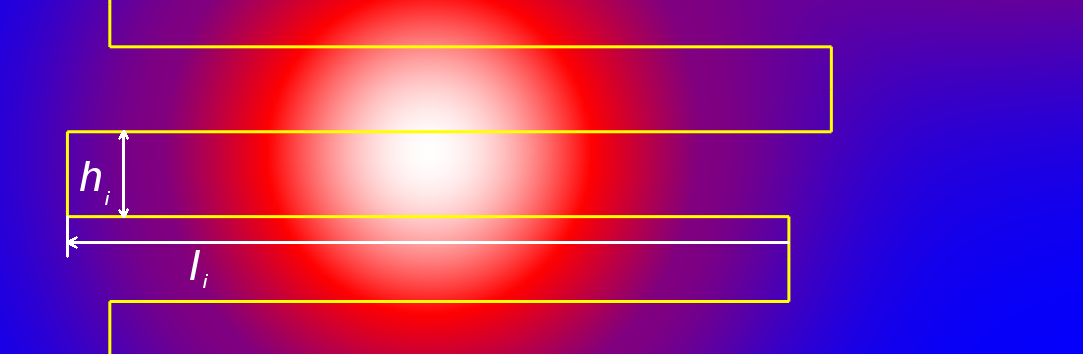
\includegraphics[width=\textwidth]{pics/pic06-lh.png}
\begin{itemize}
  \item $l_i$ --- проекция $i$-го галса на прямую $l$
  \item $h_i$ --- разница между галсом $i$ и $i+1$
  \item $S_{res}$ --- доля собранных частиц от начального распределения
\end{itemize}

\end{frame}

\section{Симуляция эволюции распределения} % Since this is the start of a new section, our recurring outline will appear here.

\begin{frame} 
\frametitle{Примеры моделей изменения распределения}
\begin{itemize}
\item{случайное блуждание с произвольным $\Delta t$ в качестве шага, $v \in [0, vMax]$}
\item{направленное движение в одном из фиксированных направлений}
\item{притяжение-отталкивание от фиксированных точек плоскости}
\end{itemize}
\end{frame}

\begin{frame}
\frametitle{Проблемa 1}
\begin{itemize}
  \item{ядро нужно применять раз в $\Delta t$ из физических соображений}
  \item{$\frac{1}{\Delta t} \ll 60FPS$} 
\end{itemize}
\end{frame}

\begin{frame}
\frametitle{Решение проблемы 1}
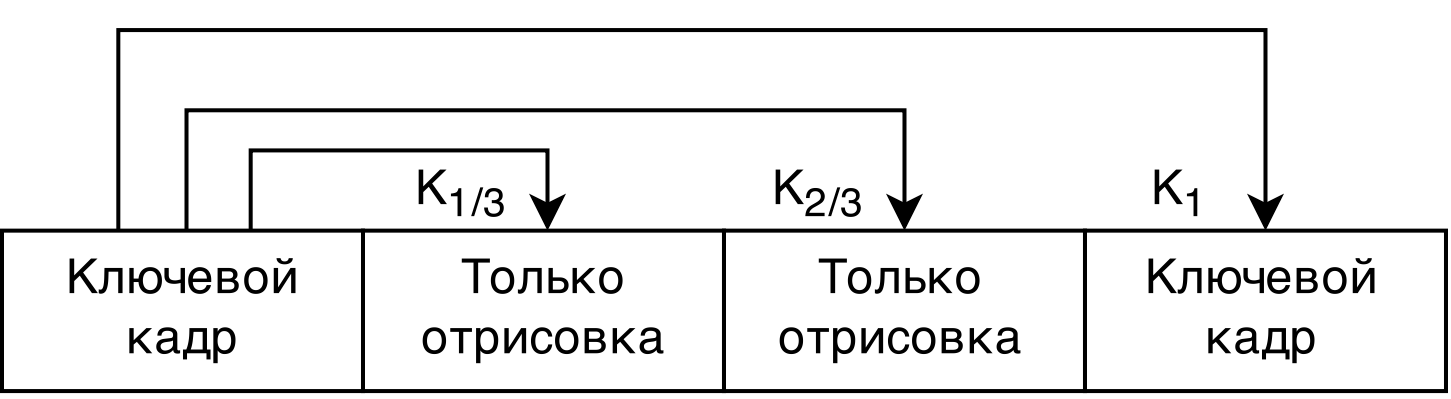
\includegraphics[width=\textwidth]{pics/keyframe.png}
\end{frame}

\section{Алгоритм построения маршрута}
\begin{frame}
\frametitle{Глобальный алгоритм}
Здесь нужно написать описание динамики за пятую степень
\end{frame}

\begin{frame}
\frametitle{Результаты работы глобального алгоритма}
\begin{columns}
\column{.6\textwidth}
\includegraphics<+>[width=\textwidth]{pics/pic01-clear.png}
\includegraphics<+>[width=\textwidth]{pics/pic01-1h.png}
\includegraphics<+>[width=\textwidth]{pics/pic01-2h.png}
\includegraphics<+>[width=\textwidth]{pics/pic01-3h.png}
\includegraphics<+>[width=\textwidth]{pics/pic01-4h.png}
\includegraphics<+>[width=\textwidth]{pics/pic01-8h.png}
\includegraphics<+->[width=\textwidth]{pics/pic01-16h.png}

\column{.4\textwidth}
\begin{itemize}
\setbeamercovered{dynamic}
\item<.(-6)>{исходное распределение}
\item<.(-5)>{1 час}
\item<.(-4)>{2 часa}
\item<.(-3)>{3 часa}
\item<.(-2)>{4 часa}
\item<.(-1)>{8 часов}
\item<.(0)>{16 часов}
\end{itemize}
\end{columns}
\end{frame}

\begin{frame}
\frametitle{Корректировка построенного пути}
\begin{columns}
\column{.6\textwidth}
\includegraphics<+>[width=\textwidth]{pics/pic02-init.png}
\includegraphics<+>[width=\textwidth]{pics/pic02-before.png}
\includegraphics<+>[width=\textwidth]{pics/pic02-after.png}

\column{.4\textwidth}
\begin{itemize}
\setbeamercovered{dynamic}
\item<.(-2)>{изначально построенный путь}
\item<.(-1)>{со временем путь устарел}
\item<.(0)>{перестроим путь}
\end{itemize}
\end{columns}

\end{frame}

\end{document}

%%% Local Variables:
%%% mode: latex
%%% TeX-master: t
%%% End:

\message{ !name(sample.tex) !offset(-279) }
